\documentclass[a4paper,12pt]{article}

\usepackage[a4paper]{geometry}

\usepackage[utf8]{inputenc}            % Use utf8 input encoding
%\usepackage[latin1]{inputenc}         % Use iso 8859-1 encoding
\usepackage[T1]{fontenc}               % T1 fonts (support for accents/diacritics)
\usepackage{lmodern}                   % font with proper T1 support and good glyph quality

\usepackage{listings}                  % for (code) listings
\usepackage{xcolor}
\definecolor{rwth}{RGB}{0 84 159}

\usepackage{listings}
\usepackage{xcolor}
\usepackage{graphicx}
\usepackage{float}

\usepackage{pgfplots}
\pgfplotsset{compat=newest}
\usepgfplotslibrary{patchplots}
\usepgfplotslibrary{dateplot}
\include{pgffor}

\lstdefinelanguage{Java}{
  morekeywords={abstract, assert, boolean, break, byte, case, catch, char, class, const,
    continue, default, do, double, else, enum, extends, final, finally, float, for,
    goto, if, implements, import, instanceof, int, interface, long, native, new,
    package, private, protected, public, return, short, static, strictfp, super,
    switch, synchronized, this, throw, throws, transient, try, void, volatile, while},
  sensitive=true,
  morecomment=[l]//,
  morecomment=[s]{/*}{*/},
  morestring=[b]",
}

\lstset{
  language=Java,
  basicstyle=\ttfamily\small,
  keywordstyle=\color{blue}\bfseries,
  commentstyle=\color{gray}\itshape,
  stringstyle=\color{orange},
  showstringspaces=false,
  numbers=left,
  numberstyle=\tiny\color{gray},
  stepnumber=1,
  numbersep=5pt,
  backgroundcolor=\color{white},
  frame=single,
  breaklines=true,
}
\usepackage{amsmath}
\usepackage{titlesec}
\usepackage{tikz}
\usetikzlibrary{automata,arrows,positioning,calc,decorations,fit,shapes,3d}

\usepackage{hyperref}

\titleformat{\section}{\LARGE\bfseries}% hide redundant number
            {}{0pt}{}

\usepackage{scalerel,stackengine}
\newcommand\equalhat{\mathrel{\stackon[1.5pt]{=}{\stretchto{%
\scalerel*[\widthof{=}]{\wedge}{\rule{1ex}{3ex}}}{0.5ex}}}}

\begin{document}

\begin{center}
	\rule{\textwidth}{0.1pt}\\[1cm]
	
	\Large Softwarepraktikum SS 2025\\\bf Assignment 2
\end{center}


\begin{center}
	\rule{\textwidth}{0.1pt}\\[0.5cm]
	{\Large Group 7\\[5mm]}
	\begin{tabular}{lll}
		David Ichim & 459591 & david.ichim@rwth-aachen.de \\
		Jenrik Meisel & 456942 & jenrik.meisel@rwth-aachen.de \\
		Jesper Nilsson & 457057 & jesper.nilsson@rwth-aachen.de \\
		Fina Schlindwein & 456038 & fina.schlindwein@rwth-aachen.de \\
	\end{tabular}\\[0.5cm]
\end{center}

\rule{\textwidth}{0.1pt}\\[1cm]

\section{Java Benchmarks}

In the previous assignment, we implemented several optimizations without thoroughly benchmarking them. We realized that making fundamental changes without proper performance comparison is not meaningful. The first thing we wanted to compare was using \texttt{byte} or \texttt{int} to store the attributes of a map like playerCount. At first we thought that \texttt{byte} was better because it uses less space, but then we noticed that we often had to explicitly cast to \texttt{byte} after doing some arithmetic calculations. To find out which version was better, we copied our \texttt{GameMap} class and replaced all occurrences of byte with int. In earlier tests we noticed that the order of the function calls had a significant impact on performance, so we tested the speed of the implementations in independent programs. To measure the time in Java, we used the following setup: \begin{lstlisting}
// setup, like parsing the map has already happend
long t1 = System.nanoTime();
SomeGameMapClass.checkAllPlacable();
SomeGameMapClass.getValidMove();
long t2 = System.nanoTime();
long timeIntBoolLayers = t2 - t1;
\end{lstlisting}
We recorded the results in a file and visualized them using plots, repeating each test multiple times to ensure statistically meaningful results.
\begin{figure}[H]
\centering
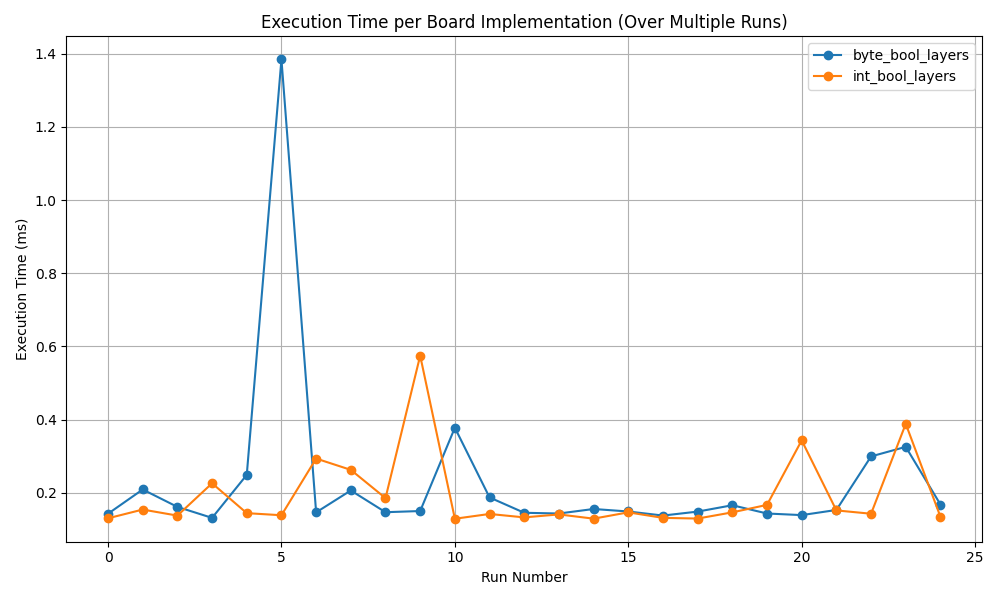
\includegraphics[width=1\linewidth]{benchmark_plots/bytevsint_original.png}
\caption{Comparison of \texttt{byte} and \texttt{int} implementations (25 iterations)}
\label{fig:25it}
\end{figure}
\begin{figure}[H]
\centering
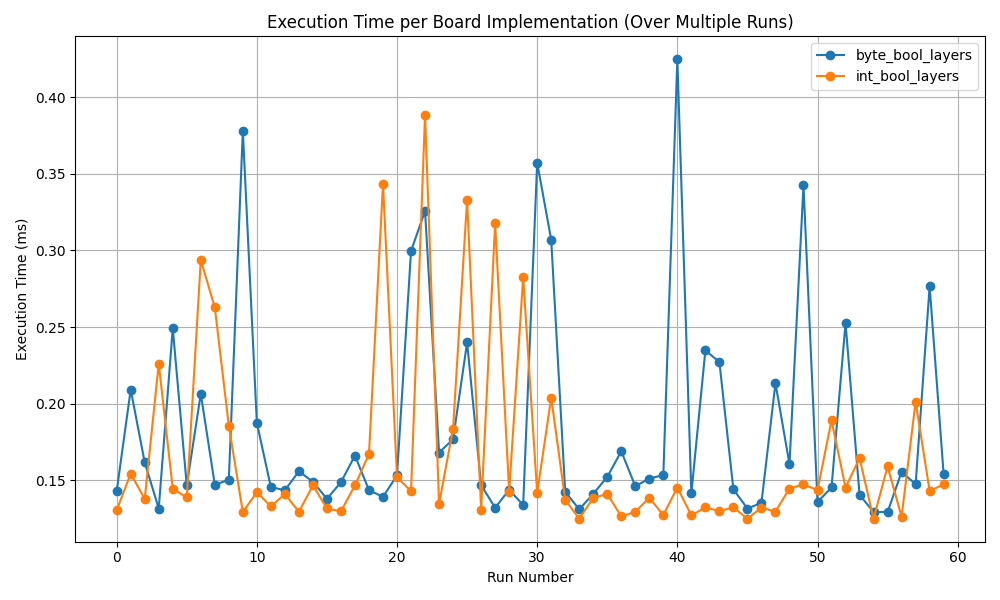
\includegraphics[width=1\linewidth]{benchmark_plots/line_longer_run.png}
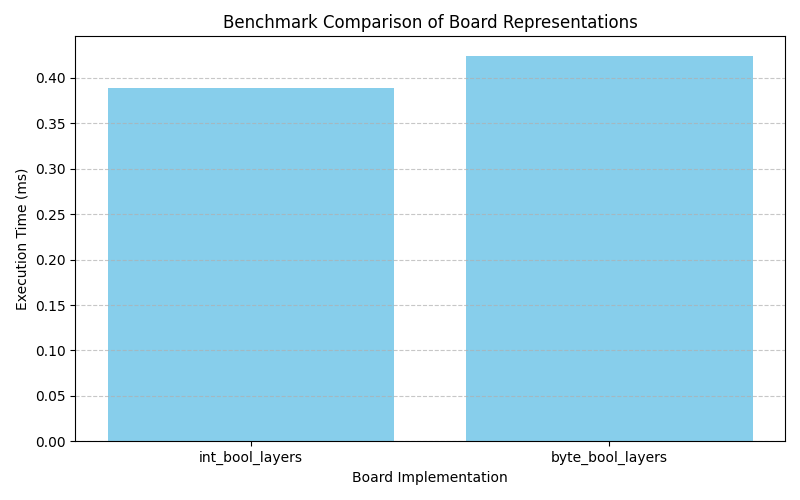
\includegraphics[width=1\linewidth]{benchmark_plots/bar_longer_run.png}
\caption{Extended comparison with 60 iterations}
\label{fig:60it}
\end{figure}
In the diagrams, the label \texttt{byte\_bool\_layers} refers to the version of the implementation that uses \texttt{byte}, \texttt{int\_bool\_layers} stands for the one that uses \texttt{int}. In the first set of tests (\autoref{fig:25it}), where each version was run 25 times, both implementations performed similarly: most executions finished in under 0.2ms. However, there were occasional spikes in execution time, making it hard to determine with implementation is faster. Those spikes might come from background activity from the JVM or some other system processes.\\[2ex]
To get a clearer picture, we ran a second round of tests with 60 iterations (\autoref{fig:60it}). This time, the results where more scattered. The increased scattering might come form external factors. We store the transitions in a hash-map, so it could also be, that a bad hash function cause some large lockup times, in some runs. \\[2ex]
Even with this variability, a trend became visible: the implementation using \texttt{int} was slightly faster on average. One likely reason is that Java automatically promotes \texttt{byte} values to \texttt{int} during arithmetic operations, and converting the results back to \texttt{byte} adds extra overhead. Besides that, using \texttt{int} also improves code readability by removing the need for repeated type casting and it becomes more clear, that we are working with numbers.\\[2ex]
Considering these points, we chose to use \texttt{int} for every number we needed to store. Although \texttt{byte} might save a small amount of memory in some scenarios, the potential gains in performance or efficiency don’t justify the added complexity.\\[2ex]
We also compared two ways of storing the map: \texttt{int[][]} and \texttt{boolean[][][]}. For a $50 \times 50$ map with the first variant we would use a \texttt{int[50][50]} array and store a number from 0 to 13 in each tile corresponding to what's on that tile. In the second case we would use an \texttt{boolean[16][50][50]} array, where we have a layer for each player and special tile. The bits set in each layer represent the occurrences of that player or special piece. We have also reserved two other layers for the valid normal moves and the valid override moves. \\[2ex]
Here we used a different approach because we wanted to increase the number of function calls to get a more rigorous result (10000 function calls). We wrote a loop, where we randomly chose which implementation we use and measured the execution time. At first we got the following graphs:
\begin{figure}[H]
\centering
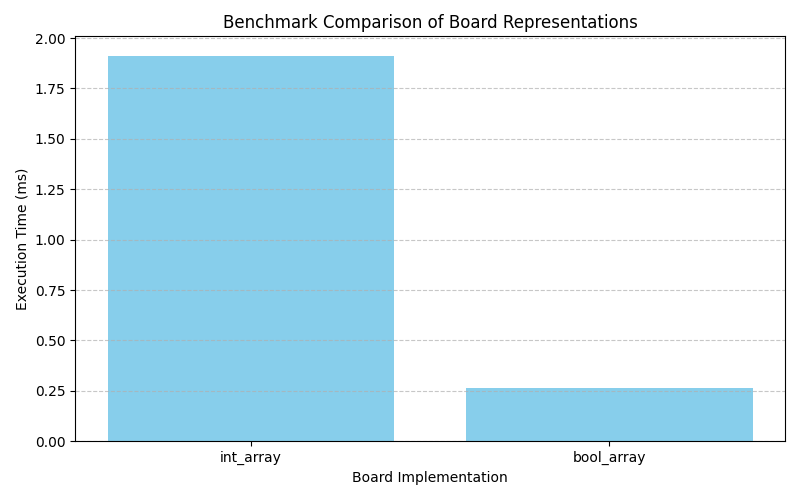
\includegraphics[width=1\linewidth]{benchmark_plots/bar_firsttry.png}
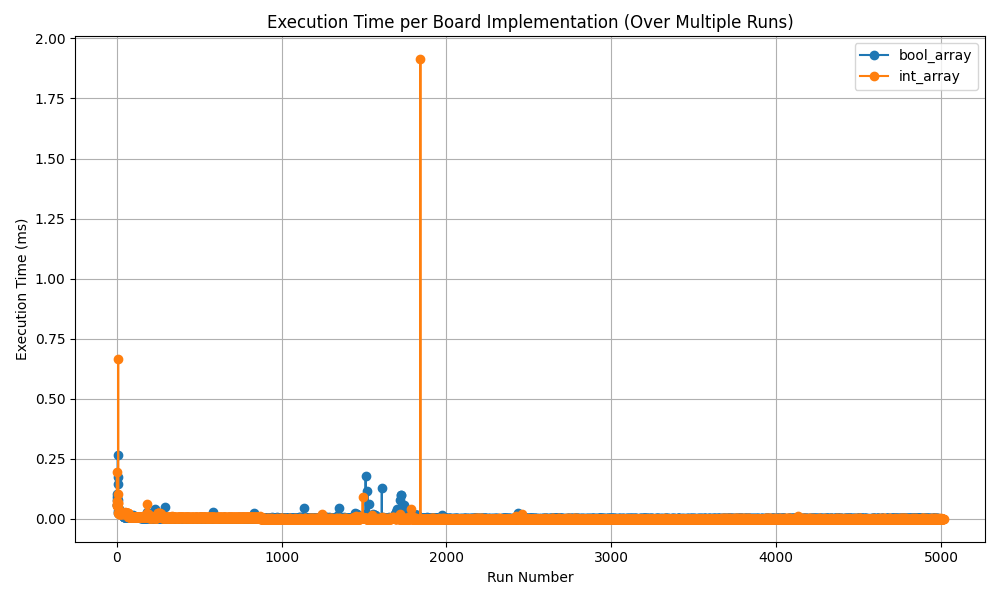
\includegraphics[width=1\linewidth]{benchmark_plots/line_firsttry.png}
\caption{First comparison, approx. 5000 iterations per Implementation}
\end{figure}

Locking at the bar diagram it seemed that using a boolean array was much faster, but analyzing the line graph, we spotted that there was a very bad run for the int array. We decided to work with averages to compensate for fluctuations. But we still wanted to calculate the averages multiple times. The following graphs where created out of data form 100 iterations, were each time an average of 100 function calls is taken:
\begin{figure}[H]
\centering
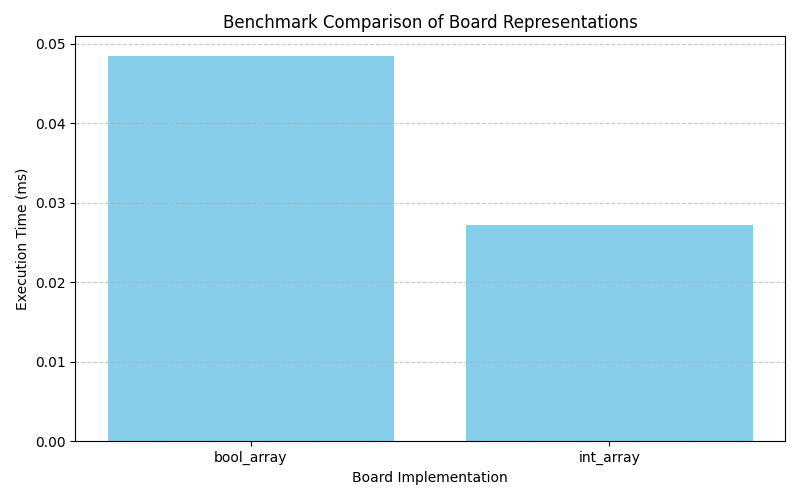
\includegraphics[width=1\linewidth]{benchmark_plots/bar_averages.png}
\caption{Comparison with averages (bar)}
\end{figure}
\begin{figure}[H]
\centering
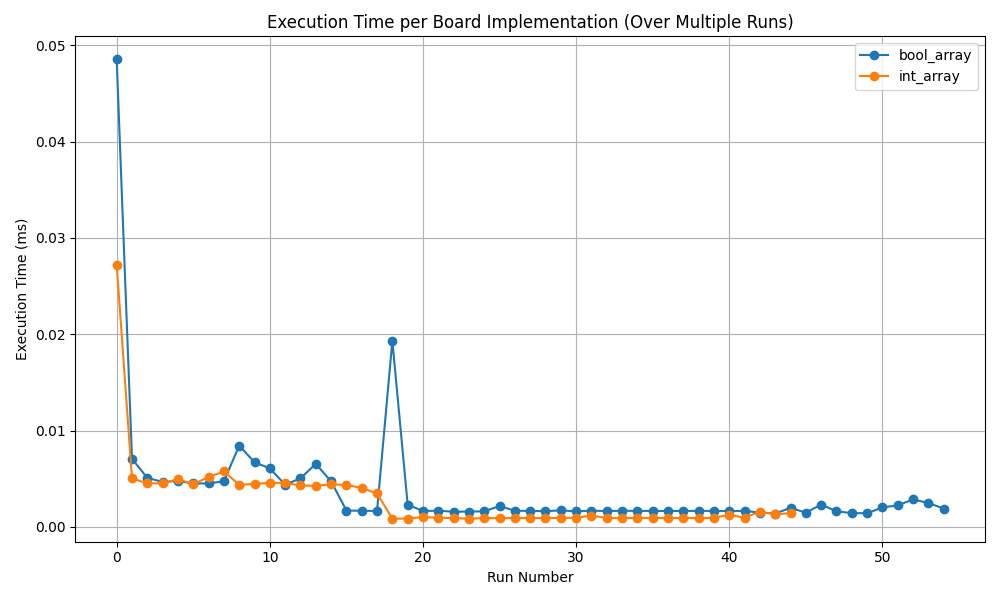
\includegraphics[width=1\linewidth]{benchmark_plots/line_averages.png}
\caption{Comparison with averages (line)}
\end{figure}
\begin{figure}[H]
\centering
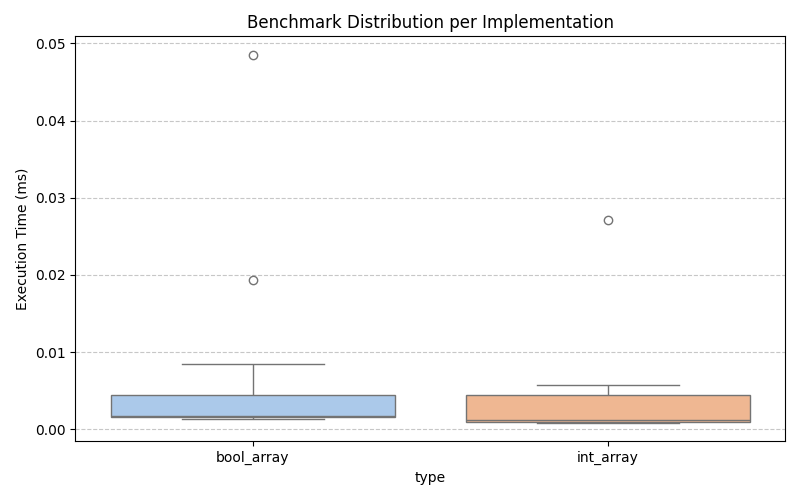
\includegraphics[width=1\linewidth]{benchmark_plots/boxplot_averages.png}
\caption{Comparison with averages (box-plot)}
\end{figure}

This time the int array performed better and the bool array had two rather bad runs. The box plots look quite similar, so it is not quite clear which version is faster.\\[2ex]
We also considered that in other maps the implementations might perform differently. So we simply ran the same code on a large map that we had downloaded from Matchpoint, this time we used 10000 iterations again, and for each iteration calculate the average of 100 function calls. The results were much clearer:
\begin{figure}[H]
\centering
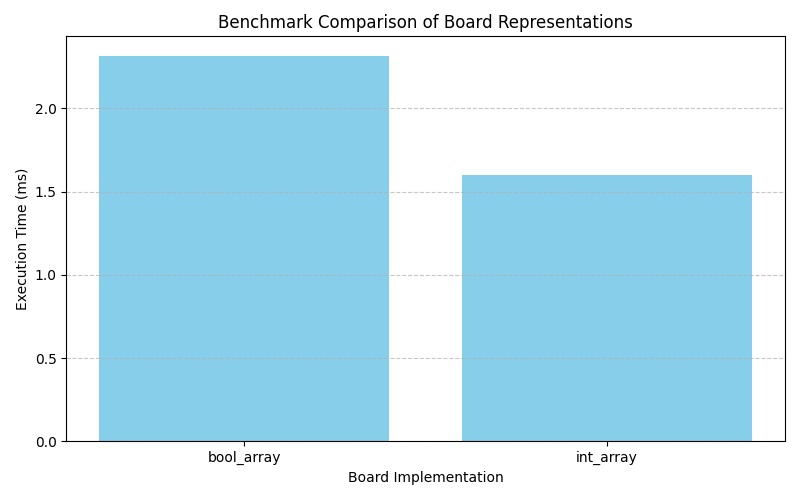
\includegraphics[width=1\linewidth]{benchmark_plots/big_map_average.png}
\caption{Comparison with averages large map  (bar)}
\end{figure}
\begin{figure}[H]
\centering
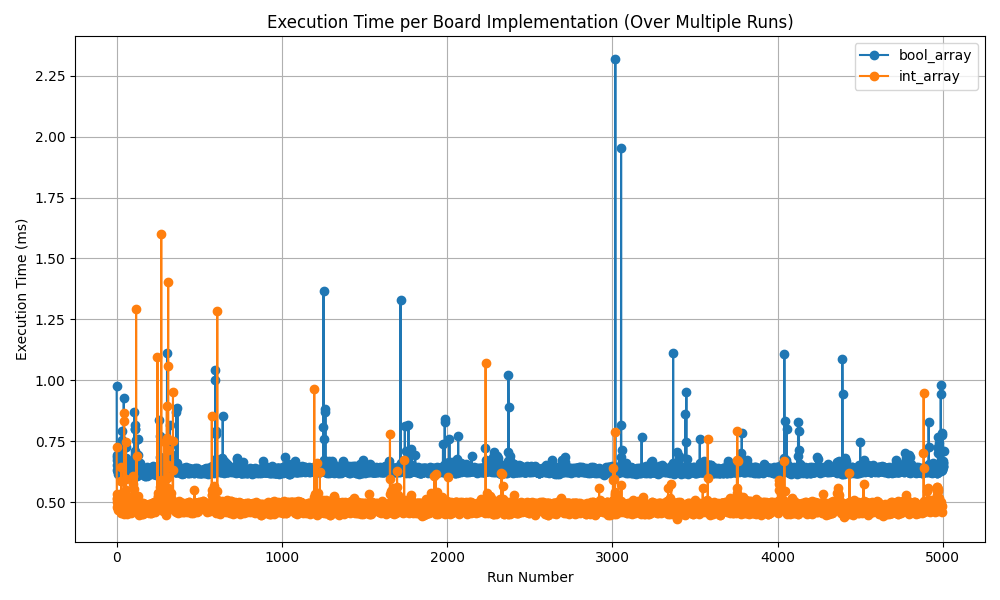
\includegraphics[width=1\linewidth]{benchmark_plots/line_big_map.png}
\caption{Comparison with averages large map (line)}
\end{figure}

All graphs show that the \texttt{int[][]} array performed better. If we look at the line we see two broad lines with a gap in between, clearly an average run with the \texttt{int[][]} array implementation was significantly faster than an average run with the \texttt{boolean[][][]} variant. To this point this was enough information to continue with the \texttt{int[][]} array.\\[2ex]
All these changes were made in Java and we found that the C++ version was still much faster. Switching to the C++ version makes the above results obsolete, but we still learned that there is absolutely no point in trying to optimise without benchmarking. In both cases, the easier to use version turned out to be the faster one.


\section{Exercise 1}

We have decided to migrate the project from Java to C++. This decision was made primarily for performance-related reasons. Benchmarking results of move generation demonstrate that our C++ implementation achieves a speedup of up to \textbf{1200x} on densely populated maps and a performance improvement of approximately \textbf{100x} on average \ref{fig:cppvsjava}. It is important to state, however, that we have devised new algorithms and employed a handful of optimizations for move generation and resolution, which massively contribute to the observed performance improvements. \\
\begin{figure}[h!]
\centering
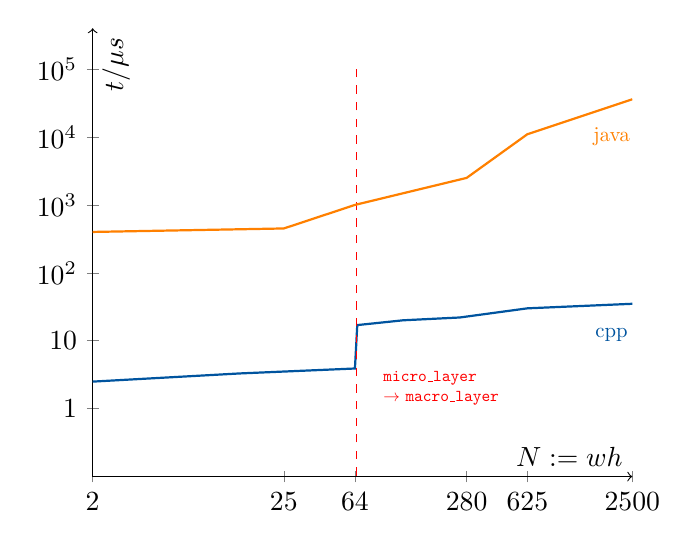
\begin{tikzpicture}[
		auto,
		semithick,
		node distance=0.0cm,
	]
	\begin{axis}[
		axis lines=left,
		axis line style={->},
		xmin=0,
		xmax=2500,
		ymin=100,
		ymax=400000000,
		xmode=log,
		ymode=log,
		log basis x=2,
		log basis y=2,
		xlabel={$N := wh$},
		xlabel style={at={(axis description cs:1,0)}, anchor=south east},
		ylabel={$t/\mu s$},
		ylabel style={at={(axis description cs:0,1)}, anchor=north east},
		xtick={2, 25, 64, 280, 625, 2500},
		xticklabels={2, 25, 64, 280, 625, 2500},
		ytick={1000, 10000, 100000, 1000000, 10000000, 100000000},
		yticklabels={1, 10, \(10^2\), \(10^3\), \(10^4\), \(10^5\)},
		grid=none,
		legend pos=outer north east
	]

	\addplot[
		color=rwth,
		thick,
	]
	coordinates {
		(2,2500)
		(14,3300)
		(64,3900)
		(66,17000)
		(121,20000)
		(256,22000)
		(625,30000)
		(2500,35000)
	};

	\draw [red, dashed] (axis cs:65,0)--(axis cs: 65,100000000);
	\node[red] at (axis cs:200,2000) [scale=0.6, align=left] {\texttt{micro\_layer} \\ \(\to\) \texttt{macro\_layer}};
	\node[rwth] at (axis cs:1900,12000) [scale=0.75, align=left] {cpp};
	\node[orange] at (axis cs:1900,10000000) [scale=0.75, align=left] {java};

	\addplot[
		color=orange,
		thick,
	]
	coordinates {
		(2,400000)
		(25,450000)
		(64,1000000)
		(280,2500000)
		(625,11000000)
		(2500,36000000)
	};
	\end{axis}
\end{tikzpicture}
\caption{Move generation Benchmark C++ vs Java}
\label{fig:cppvsjava}
\end{figure} \\
Our game client encapsulates an \texttt{Instance} object responsible for modeling the ongoing instance of Reversi Plus X as managed by the server. It must therefor be able to update its internal map representation based on a given move description and the current game state. This decoupling of instances from the client will allow us to perform evaluations on game tree nodes for future assignments, as each node may be encoded as an instance.\\\\
The generation of a successor state is handeled privately inside of the \texttt{Instance} class and is invoked via the \texttt{apply\_move} member function. The capture logic relies on the Kogge-Stone parallel prefix algorithm, using direction-specific bitshifts to avoid noise when shifting that is caused by edge-wrapping. These bitshifts rely on masks, which are precomputed and stored inside a lookup table (LUT) prior to server connection, enabling constant-time shifting in all directions, despite the boards variable size. To handle transitions on the board, the \texttt{apply\_move} algorithm checks whether a transition domain is touched during propagation in the transition domain direction. Upon detection of a possible transition, a recursive call is made to the propagation function in the transition codomain direction where the transition codomain tile on the board is set to the player's stone currently performing the capture. Resultingly, the uniform complexity of our algorithm is
\begin{align*}
	\mathcal{O}\left(T \cdot \log_2\left(\max\left\{w, h\right\}\right)\right),
\end{align*}
where \(T\) is the maximum transition depth and \(w, h\) denote the width and height of the map, respectively.\\\\
To manage the effect of inversion and choice tiles while avoiding unnecessary copies of bit layers, we map each player to a color using a fixed size array, where entry \(i\) represents the current color of player \(i\). This enables the instance to realize the effects of special tiles using simple swap operations on array elements of trivial types.\\\\
For phase 2, a routine which decomposes the bit layer map representation into an \textbf{Octree} was considered, as it allows for efficient flooding algorithms to be employed when computing the area-of-effect of bombs. We plan on further exploring this idea in the following assignments.

\section{Exercise 2}

To enable full gameplay, the client's \texttt{Instance} object must manage all player colors, override stones, bombs as well as the game phase. We used the array described in Exercise 1 (which manages player-specific values) for mapping players stones to a given color, and an array of C-style structs for keeping track of override stones and bombs of each player. When it is our client's turn to make a move, we apply it internally before yielding to the server, maximizing the time our client has for move generation on it's next turn, as it may commence searching directly. To update the map based on an opponent move notification, we extend our client to decode data received from the server to a \texttt{Move} object containing all information relevant for applying the move internally.

\section{Exercise 3}

We chose to implement the following heuristics:

\begin{enumerate}
    \item \textbf{Mobility Heuristic (1)} \\
    This heuristic evaluates the mobility of a player by calculating the number of legal moves available. It compares this number to the average number of legal moves available to all opponents. The function returns a positive value if the player's mobility is above average, and a negative value if it is below average. Here we evaluate, that the larger the return value, the better it is. Having a negative value returned signals us being below average and is not that great. The implementation is as follows:
    \begin{lstlisting}
evaluate_movement(player):
    map = get the current map variant

    // Legel moves are either normal or override moves
    Get legal moves for the player
    player_movement = count of player_normal_moves

    if player has override stones:
        player_movement += Sum of player_override_moves

    opponent_movement = 0

    for each other_player in all players:
        Get legal moves for the given player
        opponent_movement += count of opponent_normal_moves

        if other_player has override stones:
            opponent_movement += 
                Sum of opponent_override_moves

    average_opponent_movement = 
        opponent_movement / (number of players - 1)

    return player_movement - average_opponent_movement
    \end{lstlisting} 

    \item \textbf{Domination Heuristic (2)} \\
    This heuristic returns a percentage between 0 and 100 representing how many of the placed tiles are owned by the player. As percentages work, 100 is the best and 0 is the worst case. It is calculated as follows:
    \begin{lstlisting}
evaluate_domination(player):
    player_pieces = Sum of bits set in the player's map layer 

    // Build a layer containing only opponent tiles
    opponent_tiles_layer = opponent_layer(player) NAND expansion_tile
    total_pieces = Sum of bits set in opponent_tiles_layer

    if total_pieces is 0:
        return 0
 
    return (player_pieces / total_pieces) * 100
    \end{lstlisting}

    \item \textbf{Positional Heuristics: Corners and Clustering (3 \& 4)} \\
    These two related heuristics are combined into a single function. The first part evaluates the number of border edges or holes adjacent to the player's tiles. This is important because corner tiles, similar to those in traditional Reversi, are considered valuable. The second part examines how many enemy tiles are adjacent to the player’s tiles, helping to determine if the player’s tiles are clustered (fewer enemies nearby) or spread out (more enemies nearby). For the first heuristic, we consider a large amount of holes and border edges as good and for the second we consider a (for now) undetermined number that is large but not to large, as good. This uncertainty lies in 0 meaning, we aren't adjacent to any enemies and can't take next round, while a to large number suggests that we are to spread out and can be taken from all directions. We intend to adjust the number that marks best case, as figure out, if a cluster of tiles or a greatly spread out amount of pieces is strategically better. The two heuristics are calculated as follows, and returned as a pair:
    \begin{lstlisting}
evaluate_surroundings(player):
    bit_mask = the player surroundings are set to 1 
               (for each tile, the 8 neighboring positions are set to 1)

    edge_amount = (hole_layer | game_border) & bit_mask

    enemy_amount = (all_enemy_layers | expansion_layer) & bit_mask

    return <edge_amount, enemy_amount>
    \end{lstlisting}
    \item \textbf{Inversion Threat Heuristic (5)} \\
    This heuristic evaluates the risk and opportunity associated with inversion tiles. Being near an inversion tile can be dangerous if the player controls many tiles, as an opponent might trigger it. Conversely, being near such a tile is advantageous when the player controls few tiles, or is in a position to use it. This heuristic considers all choice fields we don't pick ourselves 0 at best and negative at worst, while the inversions are weighted as the difference between us and our inversion partner. Should the heuristic return a positive value, are the chances high that we will benefit through the choice and inversion tiles, while a negative number suggests a need, to prevent others from picking those tiles. The heuristic is calculated as follows:
    \begin{lstlisting}
evaluate_special():
    int result = 0

    for all enemy players:
        result -= amount of choice tiles the enemy could place on * min(enemy_tile_amount - player_tile_amount, 0)

        result += amount of inversion tiles the enemy could place on * enemy_tile_amount - player_tile_amount

    return result;
    
    \end{lstlisting}
    
    \item \textbf{Override Stone Heuristic (6)} \\
    As a little bonus, as it seamed like something we should keep track of, we also implemented a heuristic, that simply returns how many override stones we still have left. We consider a larger number better then a smaller one.
\end{enumerate}

\section{Exercise 4}

To answer the question posed in the task, we used the matplotlib plotting library for the python programming language.\\\\
For this, we initialize the pseudo-random number generator with the \texttt{seed()} function and then randomly pick a 1 or -1 with the \texttt{choice()} function from the random library for the given N number of times. The chosen number is then added to a \texttt{value} variable to display the tendency toward heads or tails.\\
For the gathered data, we track the following things:
\begin{enumerate}
    \item total amount of heads \& tails
    \item maximum \& minimum \texttt{value}
    \item longest streak of heads \& tails
    \item iterations/coin throws where \texttt{value} 0 is reached
\end{enumerate}
The data is then displayed using two graphs (and the console). First, we plot the development of the \texttt{value} variable in regards to the coin throws, as can be see in \autoref{fig1}. Second, we plot the total amount of heads and tails in a bar graph, to display the ratio, as can be seen in \autoref{fig2}.\\\\
When experimenting with this setup, we found the following regarding the tracked parameters for increasingly high sample sizes N. The first and most important observation was the 'law of large numbers' (probability theory), as we noticed that the \texttt{value} variable tended more toward 0 for larger sample sizes, as can be seen in figures 1, 3 and 4. While \autoref{fig1} has a final value of 27, \autoref{3} and \autoref{4} have final values of -19 and 179 respectively, which is a much smaller deviation from 0, when taking sample size into account. This can be seen especially well when comparing \autoref{2}, \autoref{5} and \autoref{6}, which show the ratio being closer to 1:1 for higher sample sizes. However, it is important to mention that the deviation is only reduced when taking the sample size into account. In absolute values, the devation actually increases (179 for N = 1,000,000 and 27 for N = 1,000). This can also be observed when comparing the amount of times the \texttt{value} 0 is reached (and when) for higher sample sizes. For \autoref{fig1} the \texttt{value} 0 is reached 48 times within the 1,000 iterations. However, in \autoref{fig4} in the last 1,000 iterations, the \texttt{value} 0 is only reached 7 times.\\\\
The last two observations were that for higher sample sizes, higher and lower maximum and minimum values respectively and longer streaks are reached. In \autoref{fig1} the maximum \texttt{value} is 28 and the minimum \texttt{value} is -7, while in \autoref{fig3} they are 182 and -86 and in \autoref{fig4}, they are 576 and -732 respectively. Similarly, the longest streak for heads is 10 in \autoref{fig1} and 21 in \autoref{fig3}.\\
While both of these parameters become more extreme, they are not proportional to the higher sample sizes as higher deviations become exponentially more unlikely (as a random walk this coin throwing simulation follows a normal distribution).\\\\
Moreover, to display the observed tendency towards the \texttt{value} 0, we can also plot multiple simulations in one graph, as can be seen in \autoref{fig7}. This figure shows three simulations close to 0 and two others with a slight tendency towards heads and tails, respectively.
\\\\
Lastly, until now, we have simulated the coin throwing with an unweighted coin. However, if we were to change the probabilities even slightly in favor of heads, the tendency toward 0 is replaced with a tendency toward heads, as can be seen in \autoref{8}, \autoref{9}, \autoref{fig10} and \autoref{fig11}.

\begin{figure}
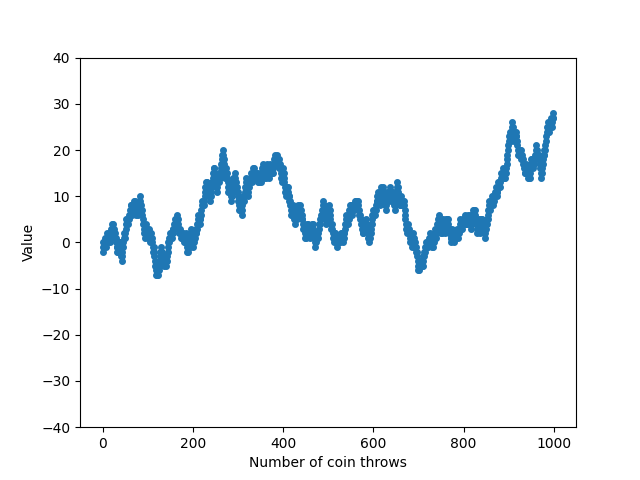
\includegraphics[scale=0.7]{./matplotlib_graphs/Figure_1.png}
\centering
\caption{Plot shows development of \texttt{value} for sample size of N = 1,000} \label{fig1}
\end{figure}

\begin{figure}
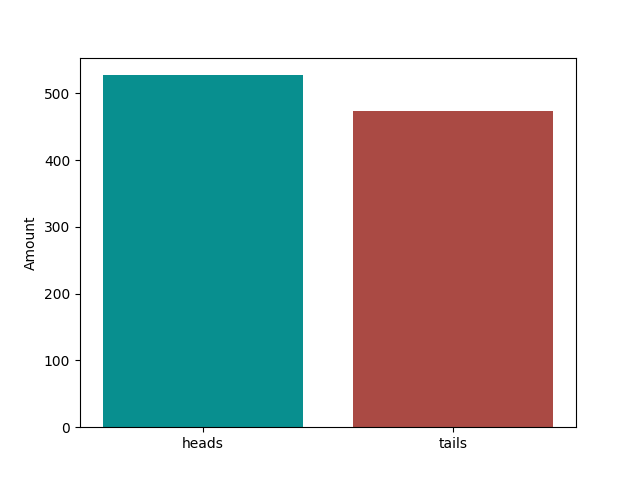
\includegraphics[scale=0.7]{./matplotlib_graphs/Figure_1_bar.png}
\centering
\caption{Bar graph shows ration of heads and tails for sample size of N = 1,000} \label{fig2}
\end{figure}

\begin{figure}
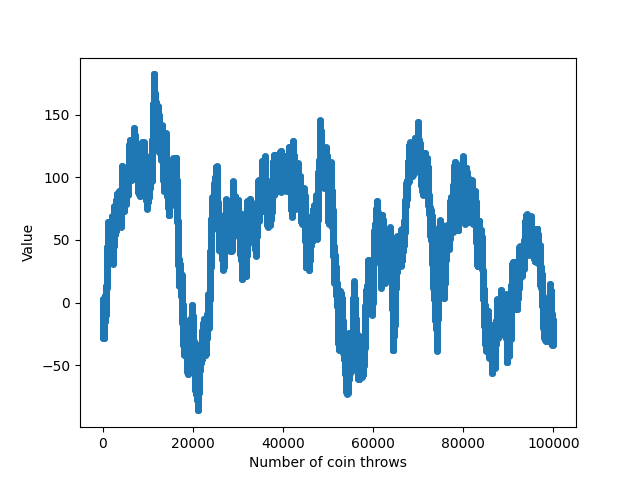
\includegraphics[scale=0.7]{./matplotlib_graphs/Figure_5.png}
\centering
\caption{Plot shows development of \texttt{value} for sample size of N = \autoref{fig10}0,000} \label{fig3}
\end{figure}

\begin{figure}
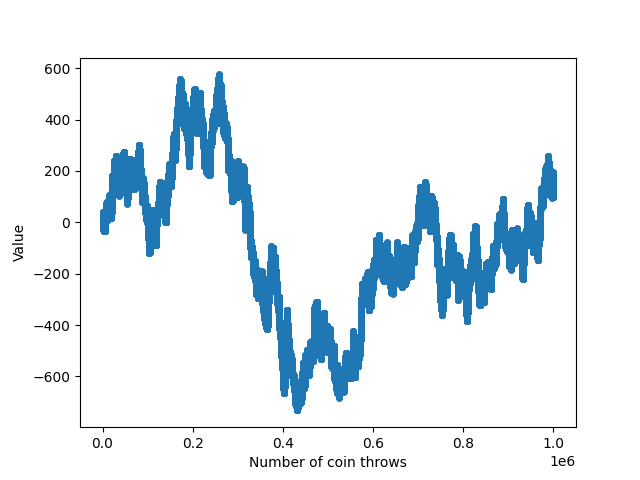
\includegraphics[scale=0.7]{./matplotlib_graphs/Figure_6.png}
\centering
\caption{Plot shows development of \texttt{value} for sample size of N = 1,000,000} \label{fig4}
\end{figure}

\begin{figure}
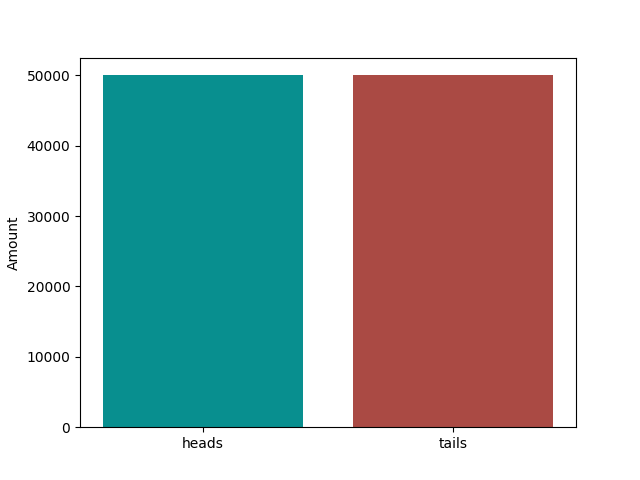
\includegraphics[scale=0.7]{./matplotlib_graphs/Figure_5_bar.png}
\centering
\caption{Bar graph shows ration of heads and tails for sample size of N = \autoref{fig10}0,000} \label{fig5}
\end{figure}

\begin{figure}
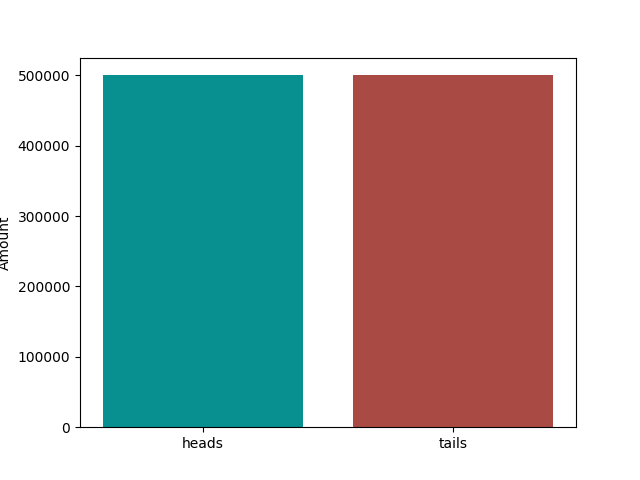
\includegraphics[scale=0.7]{./matplotlib_graphs/Figure_6_bar.png}
\centering
\caption{Bar graph shows ration of heads and tails for sample size of N = 1,000,000} \label{fig6}
\end{figure}

\begin{figure}
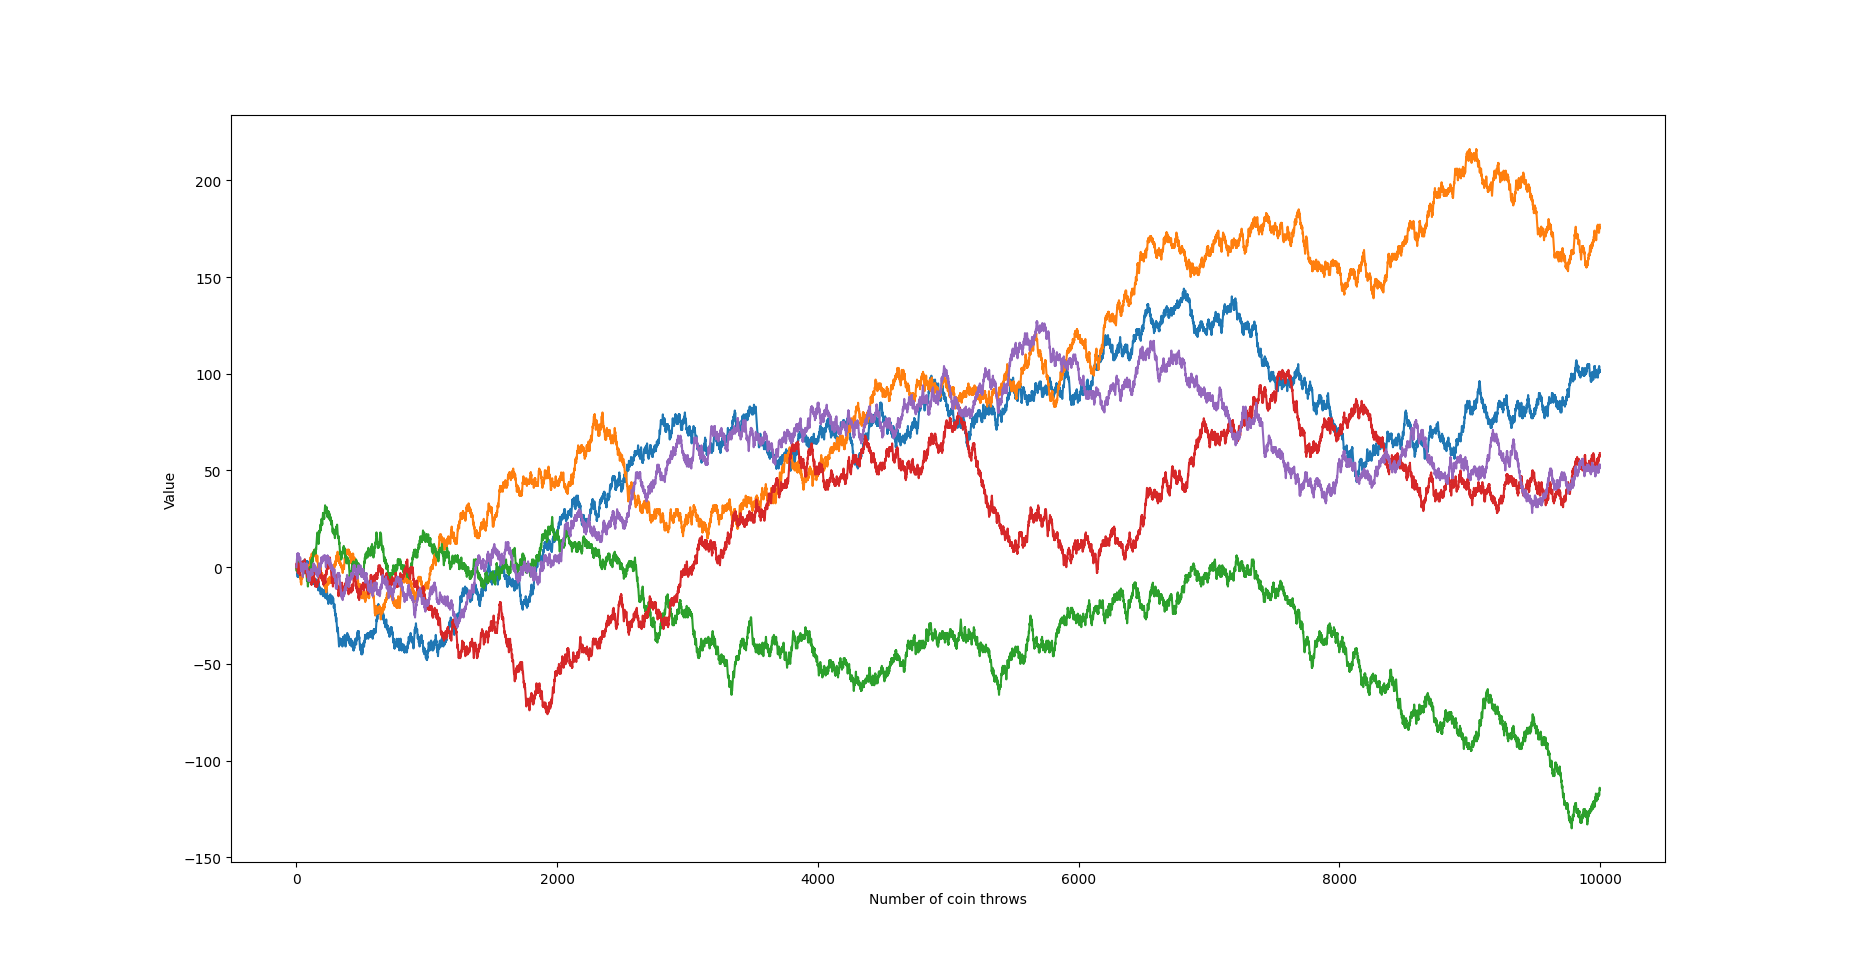
\includegraphics[scale=0.3]{./matplotlib_graphs/Figure_mult.png}
\centering
\caption{5 plots showing the development of \texttt{value} for sample size of N = \autoref{fig10}0,000} \label{fig7}
\end{figure}

\begin{figure}
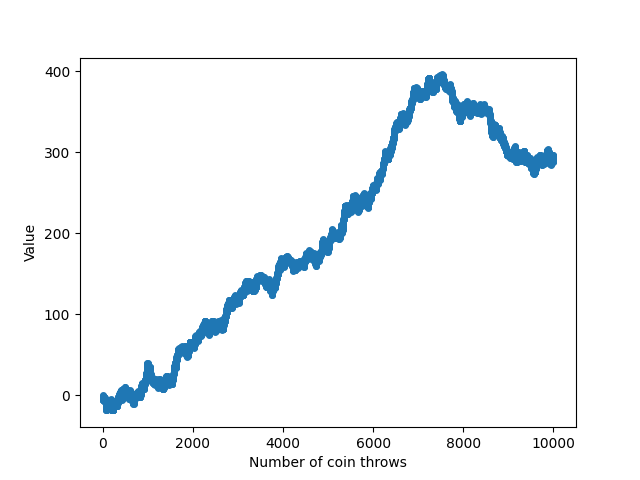
\includegraphics[scale=0.7]{./matplotlib_graphs/Figure_weighted_1.png}
\centering
\caption{Plot showing value; Probabilities: heads(0.51), tails(0.49), sample size of N = \autoref{fig10},000} \label{fig8}
\end{figure}

\begin{figure}
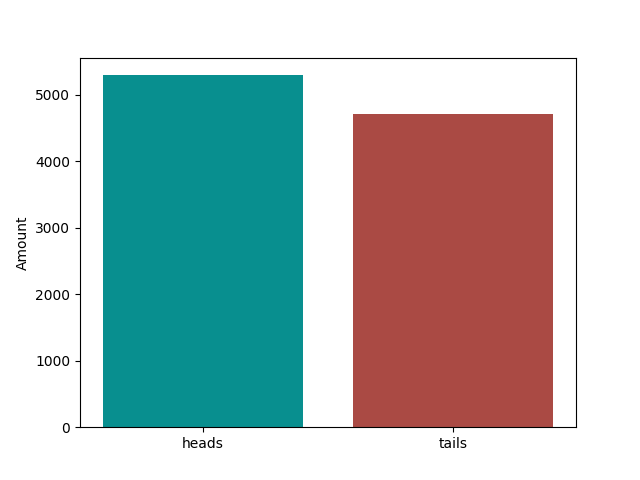
\includegraphics[scale=0.7]{./matplotlib_graphs/Figure_weighted_1_bar.png}
\centering
\caption{Bar graph showing ration; Probabilities: heads(0.51), tails(0.49), sample size of N = \autoref{fig10},000} \label{fig9}
\end{figure}

\begin{figure}
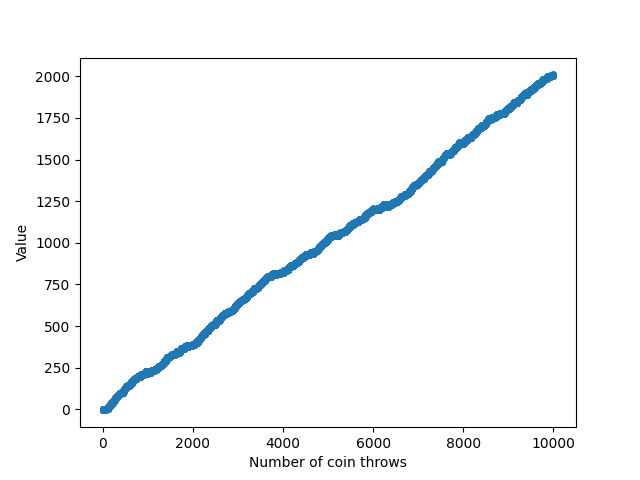
\includegraphics[scale=0.7]{./matplotlib_graphs/Figure_weighted_2.png}
\centering
\caption{Plot showing value; Probabilities: heads(0.6), tails(0.4), sample size of N = \autoref{fig10},000} \label{fig\autoref{fig10}}
\end{figure}

\begin{figure}
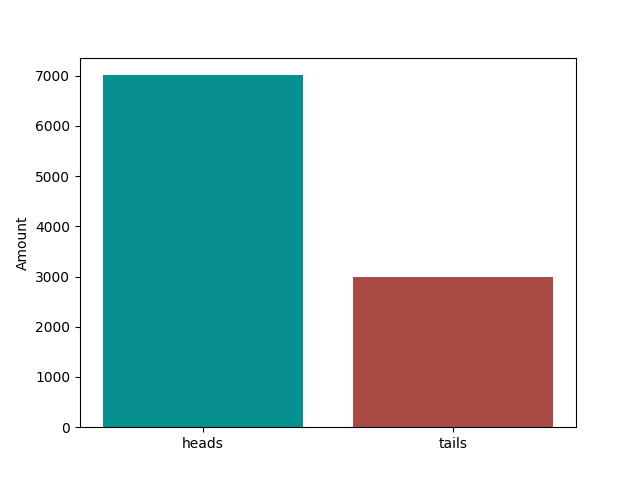
\includegraphics[scale=0.7]{./matplotlib_graphs/Figure_weighted_2_bar.png}
\centering
\caption{Bar graph showing ration; Probabilities: heads(0.6), tails(0.4), sample size of N = \autoref{fig10},000} \label{fig\autoref{fig11}}
\end{figure}



\section{Attribution}
Jenrik: Java Benchmarks, Finding Successor States \& Full Gameplay Implementation\\
Fina: Full Gameplay Implementation \& Heuristics\\
Jesper: Heuristics \& Plotting\\
David: Finding Successor States, Full Gameplay Implementation \& Heuristics

\end{document}
